%!TEX TS-program = xelatex
%!TEX encoding = UTF-8 Unicode
%!TeX spellcheck = it_IT
%!TEX root = ../tesi.tex

\chapter{Protocollo Fast Broadcast}\label{chap:protocollo-fast-broadcast}
La tecnica del Fast Broadcast~\cite{Palazzi07howdo} è nata con lo scopo di propagare un messaggio
fra veicoli utilizzando meno salti possibile; questo è reso possibile tramite una stima dinamica del raggio trasmissivo reale.
Il protcollo si compone di due fasi: la prima, chiamata ``Fase di stima'', permette a ogni veicolo di avere una stima aggiornata
del proprio raggio trasmissivo da utilizzare nella seconda fase.
La seconda, invece, è detta ``Fase di inoltro'' e viene attivata nel momento in cui si rende necessario inviare un messaggio
al resto dei veicoli presenti nell'area di interesse.
%
\section{Fase di stima}\label{sec:fb-fase-di-stima}
Durante questa fase ogni veicolo effettua una stima del suo raggio trasmissivo, sia di fronte che alle sue spalle, attraverso l'invio di messaggi \textit{Hello}.
Per ottenere una stima sempre aggiornata il tempo è suddiviso in turni e le informazioni raccolte durante un certo turno
rimangono attive per tutto il turno successivo, per poi essere scartate.
Una breve durata dei turni permette di cogliere meglio variazioni del raggio trasmissivo mantendendo tuttavia un elevato scambio di messaggi;
gli autori suggeriscono un tempo pari a un secondo.

Le informazioni sulla stima sono rappresentate dai campi \textit{Current-turn Maximum Front Range} (CMFR) e \textit{Current-turn Maximum Back Range} (CMBR).
Il primo esprime la stima della massima distanza in avanti dalla quale un altro veicolo nell'area di interesse può ricevere messaggi che provengono dal veicolo considerato.
Il secondo, invece, stima la massima distanza all'indietro.
Questi valori sono costantemente aggiornati con i valori ricevuti nei messaggi Hello fino alla fine del turno,
dopodiché vengono salvati nei campi \textit{Latest-turn Maximum Front Range} (LMFR) e \textit{Latest-turn Maximum Back Range} (LMBR) rispettivamente.
Questo permette di combinare una stima calcolata nel tempo (con diversi messaggi Hello) con le ultime informazioni sul mezzo trasmissivo.

Nel dettaglio, la procedura di invio di un messaggio Hello prevede inizialmente che il veicolo aspetti un tempo d'attesa casuale e,
dopo aver verificato l'assenza di altre trasmissioni in corso e/o collisioni, proceda all'invio del messaggio contenente
la stima del raggio trasmissivo in avanti.
Al messaggio vengono aggiunte altre informazioni utili al protocollo, come ad esempio la posizione aggiornata del veicolo.

Si fa notare che per ogni turno non più di un messaggio Hello viene inviato fra veicoli all'interno dell'area delimitata dal raggio trasmissivo.
In questo modo il numero totale di messaggi Hello generati rimane limitato nell'ordine di \BigO{1}.

In fase di ricezione, un veicolo determina la distanza fra lui e chi ha spedito il messaggio: se proviene da davanti sarà aggiornato il campo CMFR,
altrimenti se proviene dal retro verrà aggiornato il campo CMBR.
In ogni caso, la nuova stima sarà calcolata come il massimo fra il vecchio valore, la distanza fra i due veicoli e la stima inviata dall'altro veicolo
(e ricevuta nel messaggio di Hello).

Gli algoritmi~\ref{fig:algoritmo-invio-msg-hello} e~\ref{fig:algoritmo-ricezione-msg-hello} riassumono l'invio e la ricezione di un messaggio Hello.
%
\begin{italianalgorithm}[h]
\caption{Invio di un messaggio Hello.}\label{fig:algoritmo-invio-msg-hello}
\begin{algorithmic}[1]
	\ForEach{turno}
		\State{tempoInvio $\gets$ generaCasualmente(dimTurno)}
		\State{aspetta(tempoInvio)}
		\If{$\neg$ (RilevatomsgInoltro() $\vee$ RilevataCollisione())}
			\State{msgInoltro.portataMassima $\gets$ max(LMR, CMR)}
			\State{msgInoltro.posizione $\gets$ rilevaPosizione()}
			\State{inviaInBroadcast(msgInoltro)}
		\EndIf{}
	\EndFor{}
\end{algorithmic}
\end{italianalgorithm}
%
\begin{italianalgorithm}[h]
\caption{Ricezione di un messaggio Hello.}\label{fig:algoritmo-ricezione-msg-hello}
\begin{algorithmic}[1]
	\State{portata $\gets$ msgInoltro.portataMassima}
	\State{posizioneMittente $\gets$ helloMsg.posizione}
	\State{posizione $\gets$ rilevaPosizione()}
	\State{distanza $\gets$ calcolaDistanza(posizione, posizioneMittente)}
	\State{CMR $\gets$ max(CMR, distanza, portata)}
\end{algorithmic}
\end{italianalgorithm}
%
\section{Fase di inoltro}\label{sec:fb-fase-inoltro}
Lo scopo di questa fase consiste nel determinare il veicolo migliore per inoltrare un messaggio
e viene ``attivata'' nel momento in cui ci sia bisogno di propagare velocemente una certa informazione
agli altri veicoli.
Questo viene fatto sfruttando la conoscenza sulla stima del raggio trasmissivo ottenuta nella fase precedente:
ogni veicolo si assegna una priorità nell'inoltro basandosi sulla distanza dal veicolo che ha trasmesso il messaggio;
la priorità cresce all'aumentare della distanza e sarà quindi il veicolo più lontano ad avere maggiore
probabilità di effettuare l'inoltro.
La fase ha inizio con la generazione di un messaggio di \textit{Broadcast} (inoltro),
dove si trovano due valori di interesse: la posizione del veicolo e la stima del raggio trasmissivo; quest'ultima, caratteristica proprio di questo protocollo,
rappresenta quanto all'indietro ci si aspetta che arrivi il segnale prima che diventi troppo debole da non essere rilevabile.

Questo valore sarà poi sfruttato per determinare quale veicolo dovrà inoltrare il messagio in modo da minimizzare il numero di salti (\textit{hop}) e di conseguenza
ridurre il tempo di propagazione.
Nel dettaglio, quando un veicolo deve inviare o inoltrare un messaggio Broadcast calcola il valore del campo MaxRange come il massimo fra l'LMBR e il CMBR.

In fase di ricezione, un veicolo attente una quantità di tempo determinata in maniera casuale partendo dal valore di una finestra di contesa (\textit{contention window}).
Il valore di questa finestra varia fra un valore minimo (\textit{CWMin}) e un valore massimo (\textit{CWMax}), in funzione della distanza dal veicolo che ha inviato il messaggio
e la stima del raggio trasmissivo secondo la Formula~\ref{eq:contention-window}.
È facile vedere come maggiore è la distanza dal mittente e minore è l'intervallo d'attesa.
\begin{gather}\label{eq:contention-window}
	\left\lfloor \left( \frac{\text{PortataMassima} - \text{Distanza}}{\text{PortataMassima}} \times (\text{CWMax} - \text{CWMin}) \right) + \text{CWmin}  \right\rfloor
\end{gather}

Se durante l'attesa viene ricevuto lo stesso messaggio proveniente dai veicoli che seguono, ciò significa che il messaggio è già stato propagato in avanti e quindi non è necessario
che il veicolo corrente lo inoltri.
Se, invece, a inviarlo è un veicolo che precede significa che il messaggio è già stato inoltrato da un altro mezzo; la procedura quindi dev'essere fatta ripartire includendo i parametri appena ricevuti.
Nel caso in cui l'attesa finisca senza aver ricevuto nessun altro messaggio (o collisioni), il veicolo può procedere con l'inoltro includendo nell'invio la stima del raggio trasmissivo.

Gli algoritmi~\ref{fig:algoritmo-invio-msg-alert} e~\ref{fig:algoritmo-inoltro-msg-alert} riassumono quanto detto.
%
\begin{italianalgorithm}[h]
\caption{Invio di un messaggio di inoltro.}\label{fig:algoritmo-invio-msg-alert}
\begin{algorithmic}[1]
	\State{msgInoltro.portataMassima $\gets$ max(LMR, CMR)}
	\State{msgInoltro.posizione $\gets$ rilevaPosizione()}
	\State{inviaInBroadcast(msgInoltro)}
\end{algorithmic}
\end{italianalgorithm}
%
\begin{italianalgorithm}[h]
\caption{Gestione di un messaggio di inoltro.}\label{fig:algoritmo-inoltro-msg-alert}
\begin{algorithmic}[1]
	\State{cwnd $\gets$ calcolaCwnd()}
	\State{rcw $\gets$ generaCasualmente(cwnd)}
	\State{aspetta(rcw)}
	\If{stessoMessaggioDaDietro()}
		\State{esci()}
	\ElsIf{stessoMessaggioDaDavanti()}
		\State{riavviaProceduraInoltro()}
	\Else{}
		\State{msgInoltro.portataMassima $\gets$ max(LMR, CMR)}
		\State{msgInoltro.posizione $\gets$ rilevaPosizione()}
		\State{inviaInBroadcast(msgInoltro)}
	\EndIf{}
\end{algorithmic}
\end{italianalgorithm}
%
\section{Estensione a due dimensioni}\label{sec:fb-estensione-due-dimensioni}
% non mi piace molto
Nello studio originale del protocollo i veicoli erano distribuiti lungo una strada rettilinea con un singolo senso di marcia.
Ciò comportava che presi due veicoli fosse facile definirne la provenienza e la direzione, ossia chi dei due fosse davanti e chi dietro
e di conseguenza a chi inoltrare il messaggio.
Se si considera uno scenario nel quale i veicoli circolano in una rete stradale a due o più sensi di marcia,
quali sono i veicoli che si trovano davanti e quali invece dietro?
Si prenda l'esempio in \figurename~\ref{fig:v2v-1d-2d}:
se il primo veicolo a sinistra ha bisogno di propagare un messaggio il più lontano possibile,
allora è facile intuiore che a inoltrarlo dovrà essere il veicolo più a destra.
Ora invece si consideri lo scenario nell'immagine sottostante:
se è il veicolo A a dover inviare il messaggio, quale mezzo dovrà inoltrarlo, B o C?
Non è più sufficiente la differenziazione davanti-dietro.
Una soluzione a questo problema è stata proposta in~\cite{Barichello2017propagazione}:
qui la distinzione viene effettuata basandosi sulla posizione del veicolo che ha generato il messaggio.
La fase di stima non richiede modifiche sostanziali: viene eliminato il concetto di direzione e conseguentemente si utilizza solo uno dei due campi CMBR e CMFR
(creando così un CMR e un LMR).
Nella fase di inoltro, la soluzione prevede di controllare la distanza del mittente e la distanza del destinatario rispetto all'origine del messaggio.
La prima modifica necessaria è quindi la presenza nel messaggio di inoltro della posizione del veicolo che l'ha generato (oltre alla posizione del mezzo che lo inoltra).
In fase di ricezione, si controlla che la distanza origine-mezzo sia maggiore o uguale a quella origine-mittente: in tal caso il veicolo è un candidato per inoltrare il messaggio;
se così non avviene il messaggio viene scartato.
%
\begin{figure}[!h]
	\centering
		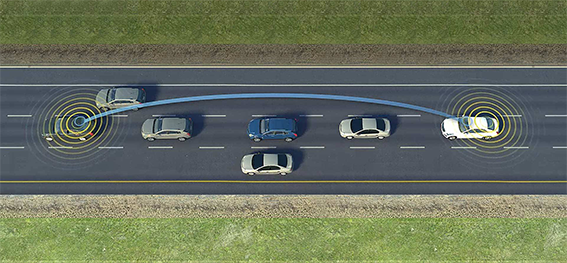
\includegraphics[width=.85\textwidth]{v2v-1d.png} \\
		\vspace{12pt}
		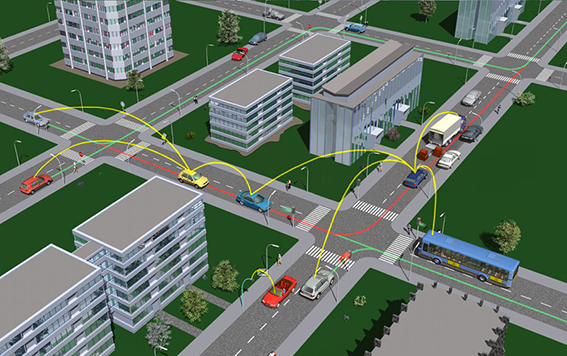
\includegraphics[width=.85\textwidth]{v2v-2d.png}
\caption{Esempio di propagazione di un messaggio in una e due dimensioni (fonte: TheDrive e Car2Car).\label{fig:v2v-1d-2d}}
\end{figure}
%
